\section{\textit{Coalition}}




O padrão arquitetural \textit{Coalition} ou coalizões trata-se de alianças que ...

%A formação de coalizões tem sido uma área muito ativa de pesquisa em SMA. A maior parte desta pesquisa concentrou-se em procedimentos descentralizados que permitem aos agentes interessados em negociar a formação de coalizões e a divisão de pagamentos de coalizões.

%O objetivo da alocação de tarefas para grupos de agentes é maximizar os benefícios por meio de seu desempenho. Buscamos um algoritmo que permita uma alocação distribuída de tarefas, ou seja, sem uma autoridade central.

%Uma baixa complexidade computacional deve ser considerada uma propriedade importante para tal solução. Assim, neste trabalho apresentamos algoritmos que permitem aos agentes formar grupos e atribuir uma tarefa a cada grupo. Nós chamamos essas coalizões de grupos. Para o desenvolvimento dos algoritmos necessários, combinamos uma abordagem algorítmica combinatória e conceitos da pesquisa operacional, com métodos de agentes autônomos e métodos de sistemas de computação distribuída.

No sistema multiagente (MAS), a coordenação e a cooperação entre os agentes são uma das questões mais importantes. Um único agente é incapaz de concluir algumas tarefas complexas porque sua capacidade é limitada individualmente ou, ainda, pode ser concluída, mas o seu desempenho e eficiência são muito inferiores ao desempenho e à eficiência com a cooperação e coordenação dos muitos agentes.

Multi-agentes com cooperação e coordenação podem ajustar metas, dissipar conflitos, compartilhar recursos para que o sistema MAS seja capaz de completar tarefas com a melhor disposição, maior eficiência e obter o maior benefício [4,5].

Portanto, a formação de coalizões é necessária quando os agentes precisam executar tarefas que não podem executar de forma eficiente sozinhos. A cooperação e coordenação entre os agentes têm uma variedade de formas.

Deles, a formação de coalizão de agentes é um dos muitos métodos importantes. No estado inicial, todos os agentes são mutuamente independentes e não cooperativos. A partir de agora, à medida que os agentes adquirem incessantemente mais conhecimento do sistema e do meio ambiente, todo agente pode formar alguma coalizão com base em certos princípios, consultando e comparando.

Cada coligação é considerada como uma totalidade independente. Todos os membros da coligação cooperam totalmente, de modo que a coligação poderá obter apoio da capacidade e dos recursos que os outros membros têm para completar tarefas por uma eficiência maior que um agente único não pode completar ou mesmo se ele puder concluir essas tarefas, a eficiência é realmente menor.

Finalmente, todo o sistema terá uma maior eficiência. No MAS, a possibilidade de cooperação mútua para a formação de coligações entre os diferentes tipos de agentes quase todos existe, e os números totais das coalizões possíveis criadas são relações exponenciais com o número de agentes no sistema MAS [2]. Para otimizar o desempenho do sistema, a possibilidade da maioria das combinações de coalizões deve ser considerada. É uma otimização combinatória complexa

\begin{description}
  \item[Nome do padrão:] \textit{} ou .
    \item[Referências:]    \citeonline{}
    \item[Categoria:] \textit{}.
    \item[Problema:] é adotado em. É adotado também para possibilitar .
    \item[Solução:] \citeonline{weiss1999multiagent} apresenta a metáfora a seguir para demonstrar este padrão.



Há, portanto, três componentes principais neste padrão \cite{dong2005event}: 

\begin{enumerate}
    \item Fontes de conhecimento (ou \textit{Knowledge Sources}): 
    \item Quadro-negro: 
    \item Controle: 
\end{enumerate}



    \item[Modelagem:] \todo{A FAZER}  %este padrão pode ser representado pela Figura \ref{fig:master_sl_diagrama_sequencia}.

\begin{comment}
\begin{figure}[h!]
    \centering
    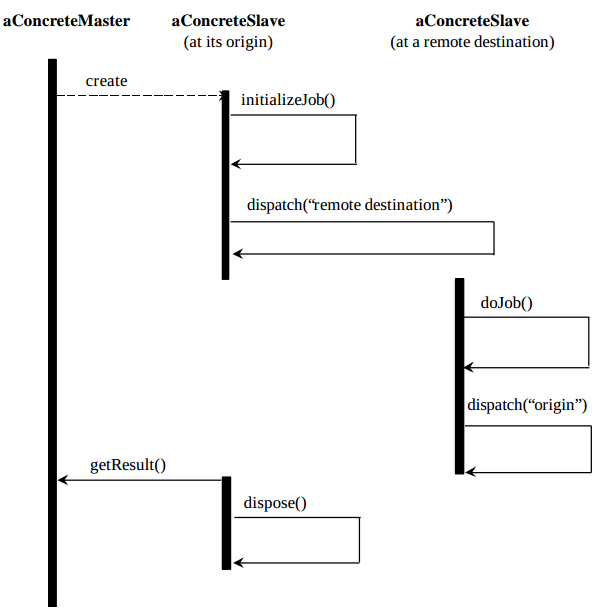
\includegraphics[scale=0.4]{figuras/master_slave/diagrama_sequencia.png}
    \caption{Diagrama de sequência do padrão \textit{Master-Slave}. Fonte: \citeonline{aridor1998agent}}
    \label{fig:master_sl_diagrama_sequencia}
\end{figure}\end{comment}


\item[Implementação:] 

De modo a exemplificar uma utilização do padrão \textit{}, é apresentado o \textit{Collaborative
Supply Chain System} (CSCS) descrito por \citeonline{ito2000blackboard}. 

Conforme mostrado na Figura \ref{fig:blackboard_example},
\begin{itemize}
    \item \textit{Intranet}:  
    \item \textit{Internet}:
\end{itemize}


\begin{figure}[h!]
    \centering
    \includegraphics[scale=0.36]{figuras/}
    \caption{. Fonte: \citeonline{}}.
    \label{fig:}
\end{figure}


\end{description}